In this lecture we devote ourselves to a discussion of classical message transmission over quantum channels. In 
Section \ref{sect:dmcqc_coding}, we discuss channel coding over a semiclassical model - channels with classical input and quantum output. We determine the message transmission of discrete memoryless channels of this type. \newline 
In Section \ref{sect:dmqc_coding}, we generalize the model to a channel with quantum input and quantum output. 
\begin{section}{The discrete memoryless  classical-quantum channel} \label{sect:dmcqc_coding}
	In this section, we assume that sender and receiver are connected  by a transmission line, where the input is a classical symbol while the output is a quantum system. This scenario is modeled by a so-called \emph{classical-quantum channel} (or \emph{cq channel})\index{channel!classical-quantum}, which is a map
	\begin{align*}
	V&: \ \cY \rightarrow \cS(\cK),  \\
	y&	 \mapsto V(y) \in \cS(\cK).
	\end{align*}
	for some alphabet $\cY$ and Hilbert space $\cK$.
	If many uses of such a channel are available in a way that the transmissions are all mutually independent, we model the transmission by the following memoryless channel model.
	\begin{definition}[Discrete memoryless classical-quantum channel] \index{DMCQC}
		The \emph{discrete memoryless classical quantum channel (DMCQC)} generated by a cq channel $V: \cX \rightarrow \cS(\cH)$ is given by the family $\{V^{\otimes n}\}_{n \in \bbmN}$
		where for each $n \in \bbmN$ the cq channel $V^{\otimes n}$ 
		\begin{align*}
		V^{\otimes n}(x^n) := \bigotimes_{i=1}^n V(x_i) = V(x_1) \otimes \cdots \otimes V(x_n)
		\end{align*}
		for each $x^n = (x_1,\dots,x_n) \in \cX^n$.
	\end{definition}
	Having defined a channel model, a standard task in information theory, is to give a general capacity formula which quantifies the message transmission abilities. We aim to determine the message transmission capacity of DMCQ channels defined above. \newline 
	A channel code for $n$ uses of a classical-quantum channel usually is given 
	by a codeword $u_m$ for each message $m$. Since the outputs of the channel are quantum mechanical systems, the decoding is performed by a quantum measurement (POVM) on the Hilbert space belonging to $n$ outputs of
	channel (a general coding scheme is depicted in Fig. \ref{fig:dmcqc_coding_pic}).
	\begin{figure}[ht] 
		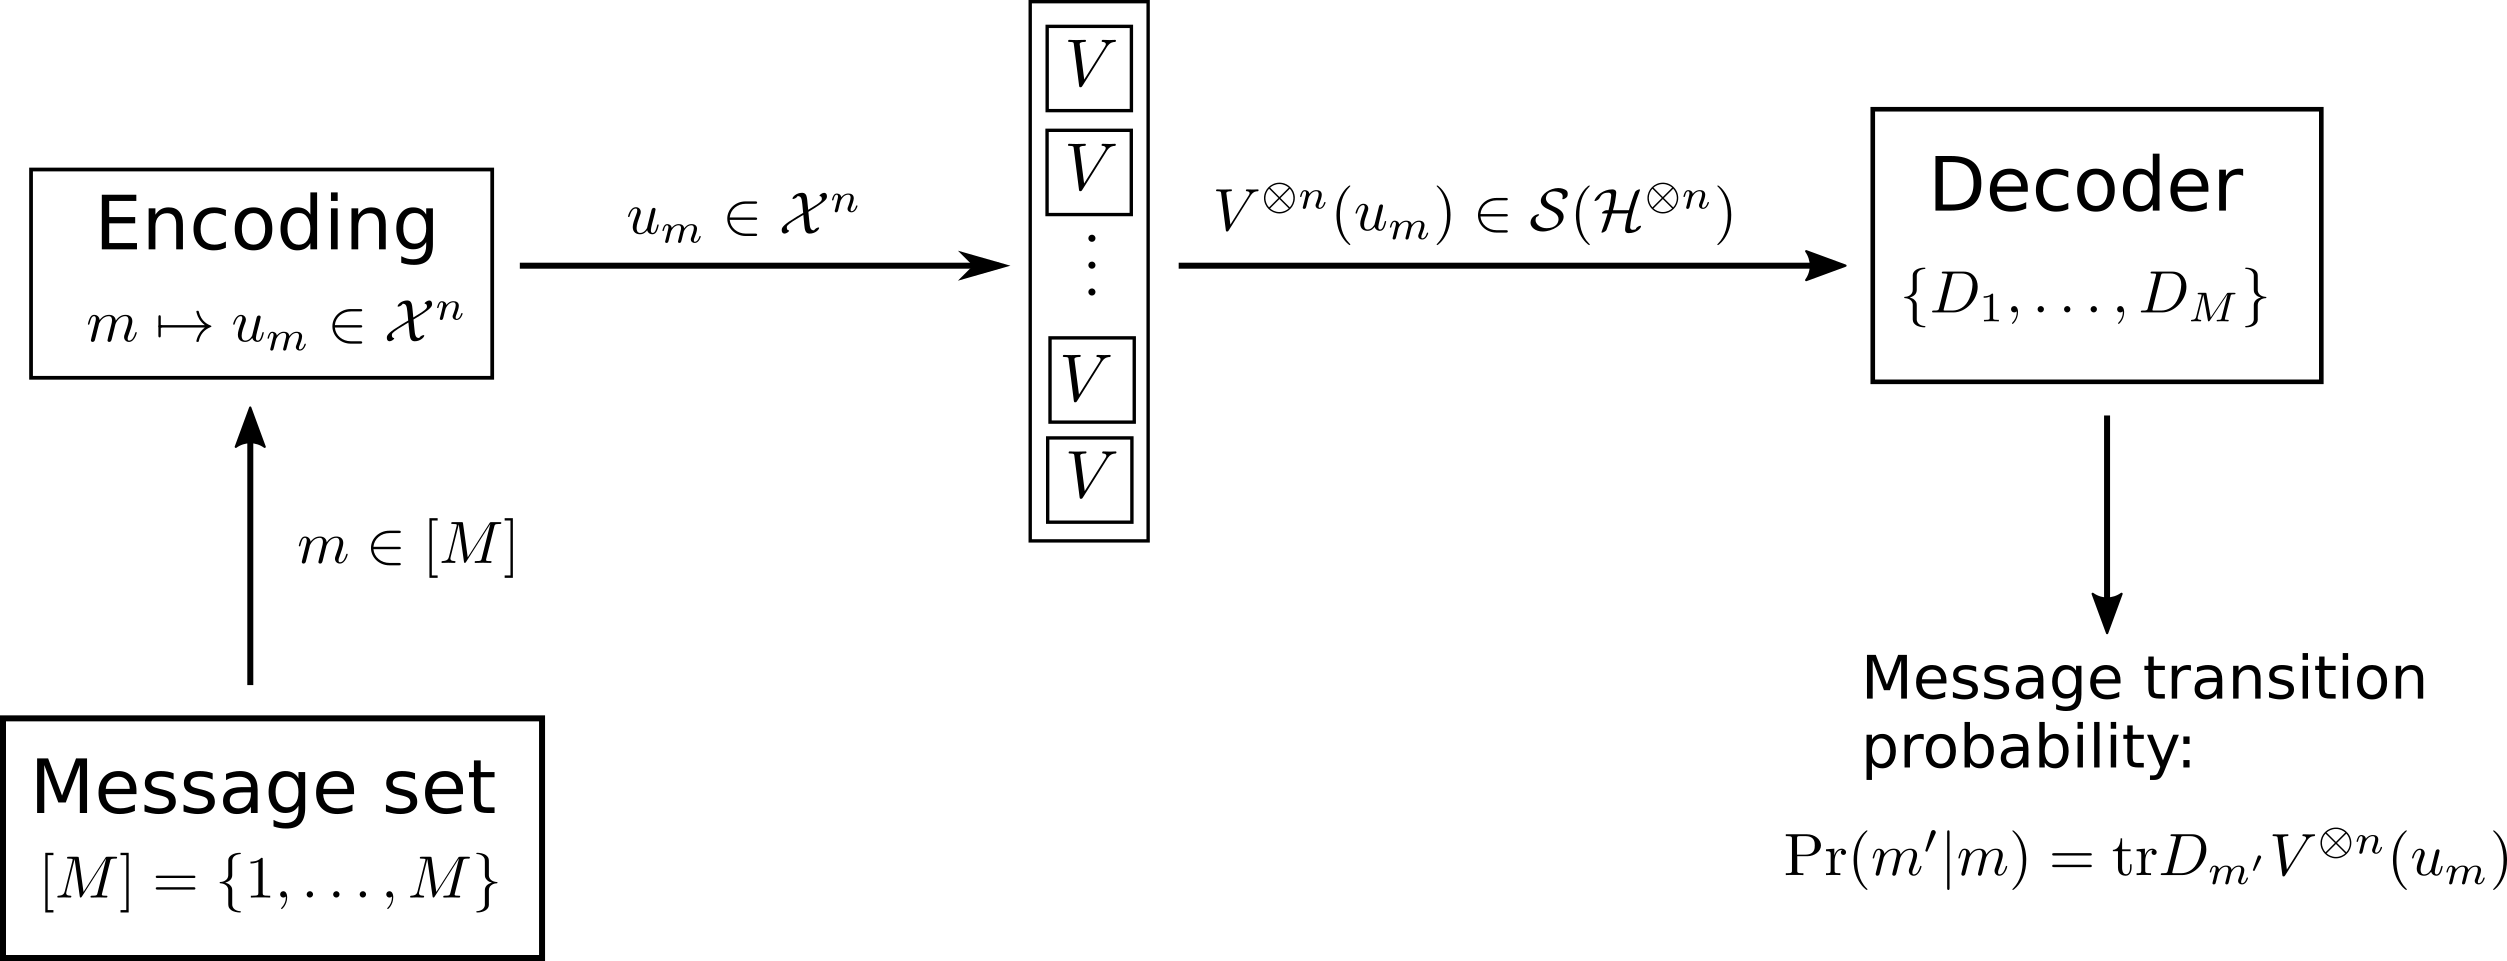
\includegraphics[width=\linewidth]{pics/dmcqc_coding_pic}
		\caption{Coding scheme for classical message transmission over $n$ uses of the DMCQC $V$.}\label{fig:dmcqc_coding_pic}
	\end{figure}
	\newpage
	We give rigorous definitions for the coding scenario. 
	\begin{definition} 
		An \emph{$(n,M)$ code for classical message transmission} over the DMCQC generated by $V: \cX \rightarrow \cS(\cH)$ is a family $\cC := (u_m,D_m)_{m=1}^M$, where 
		$u_1,\dots,u_m$ are words in $\cX^n$, and $\{D_m\}_{m=1}^M$ is a POVM in $\cL(\cH^{\otimes n})$. 
		With the shortcut $D_m^c := \bbmeins_{\cH}^{\otimes n} - D_m$, we define the functions
		\begin{align*}
		\overline{e}(\cC, V^{\otimes n}) \ := \ \frac{1}{M} \sum_{m=1}^M \ \tr D_m^c V^{\otimes n}(u_m)   &&\text{(average transmission error)}, \\
		e(\cC, V^{\otimes n}) \ := \ \underset{m \in [M]}{\max} \ \tr D_m^c V^{\otimes n}(u_m)   &&\text{(maximal transmission error)}.
		\end{align*}
	\end{definition}
	The quantities, which we aim to maximize are, for given transmission error $0 < \lambda < 1$, the maximal size of message sets for each blocklength $n$ which allow transmission error being at most $\lambda$. We define the following quantities accordingly 
	\begin{align*}
	\overline{N}(V,n,\lambda) &:= \max\{M \in \bbmN: \ \exists \ (n,M) \ \text{code} \ \cC \ \text{with} \ \overline{e}(\cC,V^{\otimes n}) \leq \lambda \}, \\
	N(V,n,\lambda) &:= \max\{M \in \bbmN: \ \exists \ (n,M) \ \text{code} \ \cC \ \text{with} \ e(\cC,W^{\otimes n}) \leq \lambda \}.
	\end{align*}
	The quantities defined above grow in general exponentially with $n$ (except, when the channel is completely useless for message transmission). We will determine the asymptotic behaviour of the \emph{transmission rates} 
	\begin{align*}
	\frac{1}{n}\log N(V,n,\lambda), \hspace{.3cm} \text{and} \hspace{.3cm} \frac{1}{n} \log \overline{N}(V,n,\lambda).
	\end{align*}
	\begin{exercise}
		Show, that for each $n\in \bbmN, \lambda \in (0,1)$ and each cq channel $V$, the inequality
		\begin{align*}
		N(V,n,\lambda) \leq \overline{N}(V,n,\lambda) \leq  \frac{1}{1-\sqrt{\lambda}} N(V,n,\sqrt{\lambda}) .
		\end{align*}
		holds. Hint: The left inequality follows directly from the definitions. The proof for the right inequality directly carries over from a corresponding relation for classical discrete memoryless channels.
	\end{exercise}
	For characterizing the message transmission capacity of the DMCQC we need the following function.
	\begin{definition}[Holevo quantity]
		Let $V: \cX \rightarrow \cS(\cH)$ be a cq channel and $q \in \cP(\cX)$ a probability distribution. The function
		\begin{align}
		\chi(q,V) := S(\overline{V}_q) - \sum_{x \in \cX} q(x) S(V(x))
		\end{align}
		with $\overline{V}_q := \sum_{x \in \cX} q(x) V(x)$ is called the \emph{Holevo quantity} \index{Holevo quantity} of $(q,V)$. 
	\end{definition}
	A convenient equivalent of the above expression can be given in terms of the quantum relative entropy. It holds by definition 
	\begin{align}
	\chi(q,V) = \sum_{x \in \cX} \ q(x) \ D(V(x)||\overline{V}_q). \label{altern_holevo_chi_form}
	\end{align}
	%It holds
	%\begin{align}
	%S(\overline{V}_q) - \sum_{x \in \cX} q(x) S(V(x)) 
	%& \ = \  - \tr\overline{V}_q \log \overline{V}_q - \sum_{x \in \cX} q(x) \tr V(x)\log V(x) \\
	%& \ = \ - \sum_{x \in \cX} q(x)  \tr  \left( V(x) \left( \log \overline{V}_q - \log V(x) \right) \right)
	%\end{align}
	Moreover, the \emph{Holevo Information} \index{Holevo information} of the channel $V$ is defined by
	\begin{align} \index{Holevo information}
	C(V) \ := \ \underset{p \in \cP(\cX)}{\sup} \ \chi(p,V).  \label{def:cq_holevo_information}
	\end{align}
	We will prove 
	\begin{theorem}[Coding Theorem and Converse] \label{thm:cq_capacity_theorem}
		Let $V: \cX \rightarrow \cS(\cH)$ be a cq channel. The following statements are true.
		\begin{enumerate}
			\item $\forall \lambda > 0:$ \ $\liminf_{n \rightarrow \infty} \frac{1}{n} \log N(V,n,\lambda) \ \geq \ C(V)$. \label{thm:cq_capacity_theorem_1}
			\item $\inf_{\lambda > 0}$ \ $\limsup_{n \rightarrow \infty} \frac{1}{n} \log \overline{N}(V,n,\lambda) \ \leq \ C(V)$. \label{thm:cq_capacity_theorem_2}
			%\item $\forall \lambda > 0:$ \ $\limsup_{n \rightarrow \infty} \frac{1}{n} \log \overline{N}(V,n,\lambda) \leq \sup_{p \in \cP(\cX)} \chi(p,V)$ \label{thm:cq_capacity_theorem_3}
		\end{enumerate}
	\end{theorem}
	The first statement in the above theorem is usually called the \emph{coding theorem} for the discrete memoryless classical-quantum channels, and the second claim the \emph{(weak) converse}
	to the coding theorem. \newline 
	Theorem \ref{thm:cq_capacity_theorem} determines the \emph{message transmission capacity} of a DMCQC $V$ by $C(V)$. \newline 
	In fact, the second claim above can be replaced by the stronger statement 
	\begin{enumerate}
		\item [2'.]$\forall \lambda > 0: \ \limsup_{n \rightarrow \infty} \frac{1}{n} \log \overline{N}(V,n,\lambda) \leq \sup_{p \in \cP(\cX)} \chi(p,V)$, \label{thm:cq_capacity_theorem_3}
	\end{enumerate}
	which is usually called the \emph{strong converse} to the coding theorem for the DMCQC. The claim in 2'. does also hold, but we will not give a proof of this statement here. 
	\subsection{The weak converse to the coding theorem}
	In this section, we aim to show the weak converse, i.e. the upper bound in Theorem \ref{thm:cq_capacity_theorem}.\ref{thm:cq_capacity_theorem_2}. To show an instance of a \emph{data processing inequality} for the Holevo quantity, we need 
	\begin{theorem}\label{cptp_monot_q_rel_entr}
		Let $\rho, \sigma \in\cS(\cH)$, and $\cN \in \cC(\cH,\cK)$. It holds
		\begin{align}
		D(\rho||\sigma) \ \geq \ D(\cN(\rho)|| \cN(\sigma)). \label{cptp_monot_q_rel_entr_1}
		\end{align}
	\end{theorem}
	The monotonicity of the quantum relative entropy under c.p.t.p. maps (inequality in Eq. (\ref{cptp_monot_q_rel_entr_1})) is provided with a very natural interpretation by Quantum Stein's Lemma (Theorem \ref{thm:q_stein_lemma}). 
	The relative entropy $D(\cN(\rho)|| \cN(\sigma))$ determines the optimal second kind error rate for quantum hypothesis tests with null hypothesis $\rho$ and alternative hypothesis $\sigma$. This rate cannot be improved by affecting both hypotheses with "noise" (that is action of a c.p.t.p. map $\cN$). This interpretation also is the idea behind the following "information-theoretic" proof of Theorem \ref{cptp_monot_q_rel_entr}
	\begin{proof}[Proof of Theorem \ref{cptp_monot_q_rel_entr}]
		We assume that $\ker \sigma \subset \ker \rho$. Otherwise $D(\rho||\sigma)$ is infinte which makes the inequality in (\ref{cptp_monot_q_rel_entr_1}) trivial. Since $\cN$ is a linear map, it also holds 
		$\ker \cN(\rho) \subset \ker \cN(\sigma)$ which ensures us, that both sides of the inequality in (\ref{cptp_monot_q_rel_entr_1}) are finite. \newline 
		We first show the inequality 
		\begin{align}
		\beta_{\epsilon, n } (\rho, \sigma) \leq \beta_{\epsilon, n } (\cN(\rho), \cN(\sigma))
		\end{align}
		for each $n \in \bbmN, \epsilon > 0$. 
		Let $\cN_\ast$ be the Hilbert-Schmidt adjoint \index{adjoint!of a c.p. map} to $\cN$ (remember Exercise \ref{ex:h_s_adjoint}). Because $\cN_\ast$ is a completely positive and unital map, the image of the set
		\begin{align}
		[0,\bbmeins_\cK^{\otimes n}] := \{a \in \cL(\cK)^{\otimes n}: \ 0 \leq a \leq \bbmeins_{\cK}^{\otimes n} \},
		\end{align}
		is contained in $[0, \bbmeins_\cH^{\otimes n}]$. We can estimate 
		\begin{align}
		\beta_{\epsilon, n}(\cN(\rho), \cN(\sigma)) 
		&= \inf\left\{\tr(\cN(\sigma)^{\otimes n} a): \ a \in [0,\bbmeins_\cK^{\otimes n}] \ \wedge \ \tr(\cN(\rho)^{\otimes n} a) \geq 1- \epsilon\right\} \nonumber \\
		&= \inf\left\{\tr(\sigma^{\otimes n} \cN^{\otimes n}_\ast(a)): \ a \in [0,\bbmeins_\cK^{\otimes n}] \ \wedge \ \tr(\rho^{\otimes n} \cN^{\otimes n}_\ast(a)) \geq 1 - \epsilon \right\} \nonumber \\
		&= \inf\left\{\tr(\sigma^{\otimes n} b): \ b \in  \cN_\ast([0,\bbmeins_\cK^{\otimes n}]) \ \wedge \ \tr(\rho^{\otimes n} b) \geq 1-\epsilon\right\} \nonumber \\
		&\geq \inf\left\{\tr(\sigma^{\otimes n} b): \ b \in  [0,\bbmeins_\cH^{\otimes n}] \ \wedge \ \tr(\rho^{\otimes n} b) \geq 1-\epsilon \right\} \nonumber \\
		& = \beta_{\epsilon, n}(\rho, \sigma).\label{cptp_monot_q_rel_entr_beta}
		\end{align}
		We conclude
		\begin{align*}
		D(\rho||\sigma) 
		& = - \lim_{n \rightarrow \infty} \frac{1}{n} \log \beta_{\epsilon,n}(\rho,\sigma) \\
		& \geq - \lim_{n \rightarrow \infty} \frac{1}{n} \log \beta_{\epsilon,n}(\cN(\rho),\cN(\sigma)) \\
		& = D(\cN(\rho)||\cN(\sigma)).
		\end{align*}
		The inequality above is by (\ref{cptp_monot_q_rel_entr_beta}). Both equalites are by using Quantum Stein's Lemma. 
	\end{proof}
	Before we proceed, we recall some notation from classical information theory. For a stochastic matrix $W: \cX \rightarrow \cP(\cY)$, and probability distribution $p \in \cP(\cX)$, the \emph{mutual information} \index{mutual information!classical} is defined by 
	\begin{align*}
	I(p,W) \ := \ H(pW) - H(W|p),
	\end{align*}
	where $pW \in \cP(\cY)$ is defined by $pW(y) := \sum_{x \in \cX} p(x)W(y|x)$, and 
	\begin{align*}
	H(W|p) := \sum_{x \in \cX } p(x) H(W(\cdot|x)).
	\end{align*}
	If the channel input and output in are regarded as a pair of random variables $(X,Y)$ with 
	distribution $P_{XY}(x,y) = p(x)W(y|x)$, also the notation 
	\begin{align}
	I(X \wedge Y) := H(X) - H(X|Y) \label{rule_class_transinformations}
	\end{align}
	Based on the classical mutual information, we define for each classical-quantum channel $V: \cX \rightarrow \cS(\cK)$ and probability distribution $p \in \cP(\cX)$ the so-called \emph{accessible information} \index{accessible information}
	\begin{align*}
	\vartheta(p,V) := \sup\left\{I(p, \tilde{V}_\cD): \ \cD \ \text{is a (finite-valued)} \ \text{POVM on} \ \cK \right\}
	\end{align*}
	where $\tilde{V}_{\cD}$ is defined as the effective $|\cX| \times |\cY|$ stochastic matrix with the entries being the conditional measurement results if the POVM $\cD :=  \{D_y\}_{y \in \cY}$ is applied on the channel ouputs, i.e. 
	\begin{align}
	\tilde{V}_{\cD}(y|x) := \tr D_yV(x) &&(x,y) \in \cX \times \cY. \label{channel_cod_effect_stoch_mat}
	\end{align}
	The following proposition provides us with data processing inequalities we need for the converse proof.
	\begin{proposition} \label{prop:holevo_bound}
		Let $V : \cX \rightarrow \cS(\cK)$, $p \in \cP(\cX)$. The following claims hold.
		\begin{enumerate}
			\item For each quantum channel $\cN \in \cC(\cK, \cH)$, it holds \label{prop:holevo_bound_1}
			\begin{align*}
			\chi(p,V) \geq \chi(p, \cN \circ V). &&\text{(Data processing inequality)}\label{holevo_dpi}
			\end{align*}
			\item In particular, it holds \label{prop:holevo_bound_2}
			\begin{align*} 
			\chi(p,V) \geq \vartheta(p,V). &&\text{(Holevo bound)}
			\end{align*}
		\end{enumerate}
	\end{proposition}
	\begin{proof}
		To prove the first claim, we consider the cq channel $\cN\circ V: \ \cX \rightarrow \cS(\cH)$ which arises from the concatenation of $V$ and $\cN$, i.e. 
		\begin{align*}
		\cN\circ V(x) = \cN(V(x))  &&(x \in \cX).
		\end{align*}
		Using the alternative formula (\ref{altern_holevo_chi_form}) for the Holevo quantity, we have
		\begin{align*}
		\chi(p,V) \ 
		&= \ \sum_{x \in \cX} \ p(x) \ D(V(x)||\overline{V}_p) \\
		&\geq \sum_{x \in \cX} \ p(x)\  D(\cN(V(x))||\cN(\overline{V}_p)) \\
		&= \sum_{x \in \cX} \ p(x)\  D(\cN(V(x))||\overline{(\cN\circ V)}_p) \\
		&= \chi(p, \cN \circ V).
		\end{align*}
		The first and the last equality above are by (\ref{altern_holevo_chi_form}) together with linearity of $\cN$ (i.e. $\cN(\overline{V}_p)= \overline{(\cN\circ V)}_p$). The inequality is by monoticity of the quantum relative entropy under c.p.t.p. maps (Theorem \ref{cptp_monot_q_rel_entr}). \\
		It remains to prove the second claim. Let $\cD := \{D_y\}_{y \in \cY} \subset \cL(\cK)$ be any POVM with $|\cY| < \infty$. We show the inequality
		\begin{align}
		\chi(p,V) \geq I(p, \tilde{V}_\cD).
		\end{align}
		Define a c.p.t.p. map $\hat{\cD} \in \cC(\cK, \bbmC^{|\cY|})$ by 
		\begin{align*}
		\hat{\cD}(a) := \sum_{y \in \cY} \ \tr(D_y a) \ \ket{e_y} \bra{e_y} &&(a \in \cL(\cK)).
		\end{align*}
		It holds
		\begin{align*}
		\hat{\cD} \circ V(x)  \ 
		&= \ \sum_{y \in \cY} \ \tr(D_y V(x)) \ \ket{e_y} \bra{e_y} \\
		&= \ \sum_{y \in \cY}  \tilde{V}_{\cD}(y|x) \ \ket{e_y} \bra{e_y}.
		\end{align*}
		Therefore, it holds (remember the definition in (\ref{channel_cod_effect_stoch_mat}))
		\begin{align}
		\chi(p,V) \
		& \geq \ \chi(p, \hat{\cD}\circ V) \nonumber \\
		& =  \ S\left(\sum_{x \in \cX} p(x) \sum_{y \in \cY}  \tilde{V}_{\cD}(y|x) \ \ket{e_y} \bra{e_y}\right) - \sum_{x \in \cX} p(x) S\left(\sum_{y \in \cY}  \tilde{V}_{\cD}(y|x) \ \ket{e_y} \bra{e_y}\right) \nonumber \\
		& = \ H(p\circ \tilde{V}_{\cD}) - H(\tilde{V}_{\cD}|p) \label{prop:holevo_bound_shannon}\\
		& =  \ I(p,\tilde{V}_{\cD}). \nonumber 
		\end{align}
		Note, that the equality in (\ref{prop:holevo_bound_shannon}) is true, because the arguments of the von Neumann entropies in the preceding line are in fact in diagonal form. 
		Maximizing over both sides of the above inequality proves the claim, we obtain
		\begin{align*} 
		\chi(p,V) \ \geq \ \sup\{ I(p,\tilde{V}_\cE): \ \cE \ \text{is a finite POVM on} \ \cH\} = \vartheta(p,V).
		\end{align*}
	\end{proof}
      The inequalities shown in the preceding proposition allow proof of some additivity properties of the Holevo quantity. 
      \begin{proposition}\label{prop:holevo-additivity}
       Let $V: \cX \rightarrow \cS(\cK)$, $W: \cY \rightarrow \cS(\cH)$ be classical-quantum channels. The following claims are true
       \begin{enumerate}
        \item $\sup_{p \in \cP(\cX \times \cY)} \ \chi(p, V \otimes W) \ = \ \sup_{q \in \cP(\cX)} \ \chi(q, V) + \sup_{r \in \cP(\cY)} \ \chi(r,W)$. \label{prop:holevo-additivity_1}
        \item For each $n \in \bbmN$, it holds \label{prop:holevo-additivity_2}
        \begin{align*}
         \frac{1}{n} \ \underset{p \ \in \cP(\cX^n)}{sup} \ \chi(p, V^{\otimes n}) \ = \ \underset{q \in \cP(\cX)}{\sup} \ \chi(q,V).
        \end{align*}
       \end{enumerate}
      \end{proposition}

      \begin{proof}
       We first show the ``$\geq$'' inequality in \ref{prop:holevo-additivity_1}. For fixed probability distributions $q \in \cP(\cX),\ r \in \cP(\cY)$, it holds with $q \otimes r$ being the notation for the product distributions to $q,r$
       \begin{align}
        \chi(q,V) + \chi(r,W) \ 
        &= \ S(\overline{V}_q) + S(\overline{W}_r) - \sum_{x \in \cX} \ q(x) S(V(x)) - \sum_{y \in \cY} \ r(y) \ S(V(y)) \nonumber \\
        &= S\left(\overline{V}_q \otimes \overline{W}_r\right) - \sum_{(x,y) \in \cX \times \cY} q \otimes r(x,y) \cdot \left(S(V(x))  + S(W(y))\right) \label{prop:holevo-additivity_s_add}\\
        &= S\left(\overline{(V \otimes W)}_{q \otimes r}\right) - \sum_{(x,y) \in \cX \times \cY} q \otimes r(x,y) S(V \otimes W(x,y)) \nonumber \\
        &= \chi(q \otimes r, V \otimes W). \label{prop:holevo-additivity_3}
        \end{align}
      The equality in (\ref{prop:holevo-additivity_s_add}) above is by additivity of the von Neumann entropy for product states (i.e. the case of equality in Lemma \ref{lemma:von_neumann_subadditivity}). Consequently, we have
      \begin{align}
       \sup_{p \in \cP(\cX \times \cY)} \ \chi(p, V \otimes W) \ 
       &\geq \ \sup_{q \in \cP(\cX)}\sup_{r \in \cP(\cY)} \chi(q \otimes r, V \otimes W) \nonumber \\ 
       &= \ \sup_{q \in \cP(\cX)} \ \chi(q, V) + \sup_{r \in \cP(\cY)} \ \chi(r,W). \label{prop:holevo-additivity_4}
      \end{align}
      The inequality above is by restricting the set for maximization. The equality follows by maximizing over the equality in (\ref{prop:holevo-additivity_3}). \newline 
      To show the reverse inequality, fix a probability distribution
      $p \in \cP(\cX \times \cY)$. We denote the marginal distributions on $\cX$ and $\cY$ deriving from $p$ by $q$ and $r$, i.e. we set
      \begin{align*}
       q(x) := \sum_{y \in \cY} \ p(x,y) \hspace{.3cm} \text{and} \hspace{.3cm} r(y) := \sum_{x \in \cX} \ p(x,y) 
      \end{align*}
      for each $x \in \cX, y \in \cY$. 
      It then holds 
      \begin{align*}
       \tr_{\cH} \overline{(V \otimes W)}_p \ = \sum_{(x,y) \in \cX \times \cY} \ p(x,y) \ \tr_{\cH}(V(x) \otimes W(y))  = \sum_{x \in \cX} \ q(x) \ U(x) = \overline{V}_q.
      \end{align*}
      By an analogous calculation, the equality 
      \begin{align*}
       \tr_{\cK} \overline{(V \otimes W)}_p = \overline{W}_r
      \end{align*}
      becomes clear. By the above equalities and subadditivity of the von Neumann entropy (Lemma \ref{lemma:von_neumann_subadditivity}), it holds
      \begin{align}
       S\left( \overline{(V \otimes W)}_p \right) \ & \leq S(\overline{V}_q) + S(\overline{W}_r).
		\label{holevo_additivity_inbetween_1}
      \end{align}
      Moreover, we have by additivity of the von Neumann entropy for tensor product states
      \begin{align}
       \sum_{(x,y) \in \cX \times \cY} \ p(x,y) \ S(V(x) \otimes W(y))
        &= \ \sum_{(x,y) \in \cX \times \cY} \ p(x,y) \ S(V(x)) + \sum_{(x,y) \in \cX \times \cY} \ p(x,y) \ S(V(y)) \nonumber \\
        &= \ \sum_{x \in \cX } \ q(x) \ S(V(x)) + \sum_{y \cY} \ r(y) \ S(V(y)). 
        \label{holevo_additivity_inbetween_2}
      \end{align}
       Thus
       \begin{align}
        \chi(p, V \otimes W) \
        & = \ S\left(\overline{(V \otimes W)}_p\right) - \sum_{(x,y) \in \cX \times \cY} \ 	p(x,y) \ S(V(x) \otimes W(y)) \nonumber \\
        & \underset{(\ref{holevo_additivity_inbetween_1}),(\ref{holevo_additivity_inbetween_2})}{\leq} \ S(\overline{V}_q) + S(\overline{W}_r) - \sum_{x \in \cX} \ q(x) S(V(x)) - \sum_{y \in \cY} \ r(y) S(W(y)) \nonumber \\
        & = \ \chi(q,V) + \chi(r,W). \label{prop:holevo-additivity_5}
       \end{align}
       Maximisation over the input probability distribution and the corresponding marginals on both sides of the inequality in (\ref{prop:holevo-additivity_5}) leads us to 
       \begin{align*}
        \sup_{p \in \cP(\cX \times \cY)} \ \chi(p, V \otimes W) \ 
       \leq \sup_{q \in \cP(\cX)}\sup_{r \in \cP(\cY)} \chi(q \otimes r, V \otimes W) 
       = \ \sup_{q \in \cP(\cX)} \ \chi(q, V) + \sup_{r \in \cP(\cY)} \ \chi(r,W),
       \end{align*}
      which shows, combined with (\ref{prop:holevo-additivity_5}) the first claim of the proposition. \newline 
      The second claim is readily verified by iteratively using the first claim, i.e. 
      \begin{align*}
         \ \underset{p \ \in \cP(\cX^n)}{\sup} \ \chi(p, V^{\otimes n}) \ 
         & = \underset{q \ \in \cP(\cX)}{\sup} \ \chi(p, V) + \underset{r \ \in \cP(\cX^{(n-1)})}{\sup} \ \chi(p, V^{\otimes (n-1)}) \\
         & = 2 \cdot \underset{q \ \in \cP(\cX)}{\sup} \ \chi(p, V) + \underset{r \ \in \cP(\cX^{(n-2)})}{\sup} \ \chi(p, V^{\otimes (n-2)}) \\
         & \vdots \\
         & = n \cdot \underset{q \ \in \cP(\cX)}{\sup} \ \chi(p, V). 
      \end{align*}
      \end{proof}
      The next lemma is well-known in classical information theory. The proof can be found in any textbook on (classical) information theory.
      \begin{lemma}[Fano's Lemma] \label{lemma:fano} \index{Fano's lemma}
       Let $(X,X')$ be a pair of random variables with values in $\cX$, and $\gamma := \prob(X \neq X')$. It holds
       \begin{align}
        H(X'|X) \ \leq \gamma \log |\cX| + h(\gamma).
       \end{align}
       with $h(t) := -t\log t - (1-t) \log (1-t)$ being the binary Shannon entropy for $t \in (0,1)$. 
      \end{lemma}
      The following proposition directly implies the weak converse statement in Theorem \ref{thm:cq_capacity_theorem} 
      \begin{proposition}\label{prop:weak_converse_inequality}
       Let $V: \cX \rightarrow \cS(\cH)$ be a classical-quantum channel. It holds
       \begin{align}
        \overline{N}(V,n,\lambda) \ \leq \ \exp \left(n \cdot C(V) + n\cdot \lambda \log |\cX| + 1 \right) \label{prop:weak_converse_inequality_1}
       \end{align}
       for each $n \in \bbmN$, $\lambda \in (0,1)$. 
       \end{proposition}
       \begin{proof}
       Let $n \in \bbmN$, $\lambda \in (0,1)$ be arbitrary but fixed. Let $\cC := (u_m,D_m)_{m=1}^M$ be any $(n,M)$-code for classical message transmission over the DMCQC $V$ which fulfills
       \begin{align}
        \overline{e}(\cC, V^{\otimes n}) \leq \lambda.
       \end{align}
       We show, that the right hand side of Eq. (\ref{prop:weak_converse_inequality_1}) is an upper bound on the number of messages in $\cC$. Let $p_{\ast} \in \cP(\cX^n)$ be the equidistribution on the set of codewords of $\cC$, i.e. 
       \begin{align*}
         p_\ast(x^n) := \begin{cases}
             \frac{1}{M} & \text{if}\ x^n \ \text{is a codeword in} \ \cC \\
             0              & \text{otherwise}
            \end{cases}
       \end{align*}
	It holds
	\begin{align}
	 n \cdot \sup_{p \in \cP(\cX)} \ \chi(p,V) \ 
	 & = \ \sup_{q \in \cP(\cX^n)}  \ \chi(q,V^{\otimes n}) \nonumber \\
	 & \geq \chi(p_\ast, V^{\otimes n}) \nonumber \\
	 &\geq \vartheta(p_{\ast}, V^{\otimes n}). \label{prf:weak_converse_inequality_1}
	\end{align}
        The equality above is by Proposition \ref{prop:holevo-additivity}.\ref{prop:holevo-additivity_2}, the last inequality follows from Holevo's bound Proposition \ref{prop:holevo_bound}.\ref{prop:holevo_bound_2}.
        Using the decoding POVM $\cD := \{D_m\}_{m=1}^M$ from $\cC$, we define a stochastic matrix $\tilde{V}_{n, \cD}: \ \cX^n \rightarrow \cP([M])$ defined by entries
        \begin{align*}
            \tilde{V}_{n,\cD}(m|x^n) := \tr V^{\otimes n}(x^n)D_m &&( x^n \in \cX^n, m \in [M]).
        \end{align*}
        Using (\ref{prf:weak_converse_inequality_1}), we obtain
        \begin{align}
         n \cdot \sup_{p \in \cP(\cX)} \ \chi(p,V) \ \geq \ \vartheta(p_{\ast}, V^{\otimes n}) \ = \underset{\cE \ \text{POVM}}{\sup} \ I(p_{\ast}, (\widetilde{V^{\otimes n}})_{\cE}) \ \geq \ I(p_{\ast}, \tilde{V}_{n,\cD}).
         \label{prf:weak_converse_inequality_2}
        \end{align}
	 Let $(X,Y)$ be the pair of random variables defined by 
	 \begin{align*}
	  \prob\left(X = m \ \wedge \ Y = m' \right) \ 
	  &= \tilde{V}_{n,\cD}(m'|x_m) p_{\ast}(x_m). 
	 \end{align*}
      Then, 
      \begin{align}
       I(p_{\ast}, \tilde{V}_{n,\cD}) \ 
       = \ I(X\wedge Y) \nonumber
        \underset{(\ref{rule_class_transinformations})}{=} H(X) - H(X|Y).
      \end{align}
      Because we chose $p_{\ast}$ to be equidistributed, it holds
      $
       H(X) = H(p_{\ast}) = \log M.
      $
       Note, that also 
      \begin{align}
       \gamma := \prob \left(X \neq Y\right) \
       &= \sum_{m=1}^M \sum_{m' \neq m} \ \prob \left(X = m \wedge Y = m' \right) \nonumber \\
       &= \sum_{m=1}^M \sum_{m' \neq m} p^n(u_m) \cdot \tr D_{m'}V^{\otimes n}(u_m) \nonumber \\
       &= \frac{1}{M} \sum_{m=1}^M \tr(\bbmeins - D_{m})V^{\otimes n}(u_m) \nonumber \\
       &= \overline{e}(\cC, V^{\otimes n}) \label{prf:weak_converse_inequality_} \nonumber \\
       &\leq \lambda
      \end{align}
      holds. Using Fano's inequality (Lemma \ref{lemma:fano}) in combination with the above equality, we further bound the right hand side of Eq. (\ref{prf:weak_converse_inequality_2}). In fact, 
      \begin{align*}
       I(p_{\ast}, \tilde{V}_{n,\cD}) \ 
       = \ H(X) - H(X|Y) \
       \geq \log M - \lambda \log M - h(\lambda).
      \end{align*}
      We end up at
      \begin{align*}
       n \cdot \sup_{p \in \cP(\cX)} \chi(p,V) \ \geq \ \log M - \lambda \log M - 1 \geq \log M - \lambda n \log |\cX| - 1,
      \end{align*}
      which can be rearranged to 
      \begin{align*}
       \log M \ \leq \ n C(V) + n \cdot \lambda \log |\cX| + 1.
      \end{align*}
      Since $\cC$ was an arbitrary code with average error bounded from above by $\lambda$, maximising $M$ over all such codes yields the claimed inequality. 
      \end{proof}
     \subsection{The coding theorem}
      In this section, we aim to show the ``achievability part'' of Theorem \ref{thm:cq_capacity_theorem}. The statement follows directly from the claim of the following proposition. 
     \begin{proposition} \label{prop:holevo_coding_theorem}
       Let $W: \cX \rightarrow \cS(\cH)$ be a cq channel. For each $\lambda \in (0,1)$, and $\delta > 0$ there is a number $n_0 := n_0(\lambda,\delta)$, such that for all $n \geq n_0$ the 
       inequality
       \begin{align*}
        \overline{N}(W,n,\lambda) \ \geq \ \exp\left(n(C(V) - \delta) \right)
       \end{align*}
       is true. 
      \end{proposition}
       One of the main "nonclassical" challenges in our proof of Proposition \ref{prop:holevo_coding_theorem} is to replace a matrix product by a sum. The following matrix inequality provides a suitable replacement for the "union bound" which would be used in the corresponding classical proof. 
      \begin{lemma}[Hayashi-Nagaoka inequality] \label{hayashi_nagaoka_ineq}
       Let $a, b \in \cL(\cK)$ be matrices with $0 \leq a \leq \bbmeins_{\cK}$, $b \geq 0$. It holds
       \begin{align}
        \bbmeins_\cK - (a+b)^{-\tfrac{1}{2}} a (a+b)^{-\tfrac{1}{2}} \ \leq 2(\bbmeins_\cK - a) + 4b, \label{hayashi_nagaoka_ineq_1}
       \end{align}
       where $y^{-1}$ is the generalized inverse of $y$.
      \end{lemma}
       \begin{proof}
        We can assume without loosing generality that $a+b$ has full rank. This can be seen as follows. Let $P$ denote projector onto the support of $a+b$. Note, that $P$ as well as $P^\perp := \bbmeins - P$ commute with $a, b, a+b$. The inequality in \ref{hayashi_nagaoka_ineq_1} holds therefore if and only if the inequalities 
        \begin{align}
        P - (a+b)^{-\tfrac{1}{2}} a (a+b)^{-\tfrac{1}{2}}P \ \leq 2P - PaP + 4PbP
        \label{hayashi_nagaoka_ineq_2}
        \end{align}
        and 
        \begin{align}
        P^\perp - P^\perp(a+b)^{-\tfrac{1}{2}} a (a+b)^{-\tfrac{1}{2}}P^\perp \ \leq 2P^\perp - P^\perp aP^\perp + 4P^\perp bP^\perp \label{hayashi_nagaoka_ineq_3}
        \end{align}       
        simultaneously hold. The inequality in (\ref{hayashi_nagaoka_ineq_3}) is in fact the trivial inequality $P^\perp \leq 2P^{\perp}$. 
        The inequality in (\ref{hayashi_nagaoka_ineq_2}) regarded as a matrix inequality on $\supp(a+b)$, i.e. a version of the original inequality in (\ref{hayashi_nagaoka_ineq_1}) where $(a+b)$ has full rank. \newline   
        First, we note, that for given matrices $x,y,w,z$ it holds
        \begin{align*}
         (x-\bbmeins)b(x - \bbmeins) \ = \ xbx - xb -bx + b, 
        \end{align*}
        which with some rearrangements leads us to 
        \begin{align*}
         xbx \ = \ b + (x-\bbmeins)b + b(x - \bbmeins) + (x - \bbmeins)b(x - \bbmeins). 
        \end{align*}
        Moreover, it holds $(w-z)^\ast (w-z) \geq 0$, which implies 
        \begin{align*}
         w^\ast z + z^\ast w \ \leq w^\ast w + z^\ast z.
        \end{align*}
        which applied with $w := \sqrt{y}(x-\bbmeins)$ and $z := \sqrt{y}$ reads 
        \begin{align}
         (x-\bbmeins)b + b(x-\bbmeins) \ \leq \  (\bbmeins - x)b(\bbmeins -x) + b \label{hn_ineq}
        \end{align}
        We set $x := (a+b)^{-\tfrac{1}{2}}$. We have   
        \begin{align*}
         \bbmeins - (a+b)^{-\tfrac{1}{2}} a (a+b)^{-\tfrac{1}{2}}  \ 
         & \ =	\	 \bbmeins - xax \\
         & \ =	\	 x(a+b)x - xax \\
         & \ =	\	 xbx \\
         & \ =	\	 b + w^\ast z + z^\ast w + (x-\bbmeins) b (x - \bbmeins) \\
         & \ \overset{(\ref{hn_ineq})}{\leq}\	 2b + 2(x - \bbmeins) b (x - \bbmeins) \\
         & \ \overset{(*)}{\leq} \	 2b + 2(x-\bbmeins)x^{-2}(x-\bbmeins) \\
         & \ = 	\	 2b + 2(\bbmeins - 2x^{-1} + x^{-2}) \\
         & \ = 	\	 2b + 2(\bbmeins - 2 (a+b)^\frac{1}{2} + a + b) \\
         & \ \overset{(**)}{\leq} \	 2b + 2(\bbmeins - 2 a + a + b) \\
         & \ = 	\	 4b + 2(\bbmeins - 2 a)
         \end{align*}
		 The equalties above are by rearrangement of terms, $(*)$ is by the inequality $b \leq (a+b) = x^{-2}$, and $(**)$ is true, because the map $x \mapsto x^{\frac{1}{2}}$ is matrix monotone, therefore $a \leq a^{-\frac{1}{2}} \leq (a+b)^{-\frac{1}{2}}$.
       \end{proof}
     Let $V: \cX \rightarrow \cS(\cH)$ be a classical-quantum channel, and $q \in \cP(\cX)$ be a probability distribution. We define density matrices $\rho(p,V)$ and $\sigma(p,V)$ on $\bbmC^{|\cX|} \otimes \cH$ by
      \begin{align}
       \rho(p,V) \ &:= \ \sum_{x \in \cX} q(x) \ket{e_x} \bra{e_x} \otimes V(x) \label{channel_cq_state_1}\\
       \sigma(p,V) \ &:= \ \sum_{x \in \cX} q(x) \ket{e_x} \bra{e_x} \otimes \overline{V}_q,      
       \label{channel_cq_state_2}
      \end{align}
      where we again used the definition $\overline{V}_q := \sum_{x \in \cX} V(x)$.
      \begin{exercise} \label{ex:cq_states_holevo_chi}
       Show, that for $V: \cX \rightarrow \cS(\cH)$, and $q \in \cP(\cX)$
       \begin{align*}
       \chi(q,V) \ = \ D(\rho(q,V)||\sigma(q,V))
       \end{align*}
       holds for the states defined in (\ref{channel_cq_state_1}) and (\ref{channel_cq_state_2}). Hint: Realise, that both matrices can be written as a Block-diagonal matrix, then use the definition of $D(\cdot||\cdot)$. 
      \end{exercise}

      \begin{proposition}[Random coding] \label{prop:coding_from_stein}
       Let $V: \cX \rightarrow \cS(\cH)$ be a classical-quantum channel, and $q \in \cP(\cX)$. Assume, we find for given $n \in \bbmN$, $\lambda \in (0,1)$, $\tau > 0$ an effect $a \in \cL(\cH \otimes \bbmC^{|\cX|})^{\otimes n}$, 
       $0 \leq a \leq \bbmeins_{\cH \otimes \bbmC^{|\cX|}}^{\otimes n}$ which fulfills the conditions
       \begin{enumerate}
        \item $\tr a \rho(q,V)^{\otimes n} \ \geq 1 - \lambda$ and 
        \item $\tr a \sigma(q,V)^{\otimes n} \leq \tau$. 
       \end{enumerate}
	Then there exists for each $M \in \bbmN$ an $(n,M)$-code $\cC = (u_m, D_m)_{m=1}^M$ with
	\begin{align*}
	 \overline{e}(\cC, V^{\otimes n}) \ < \ 2 \lambda + 4M\tau.
	\end{align*}
      \end{proposition}
      \begin{proof}
      Fix $n \in \bbmN$. We set shortcuts $\rho:= \rho(q,V)$, and $\sigma := \sigma(q,V)$. Let 
      \begin{align*}
          v: \ \left(\bbmC^{|\cX|} \otimes \cH)^{\otimes n}\right){\otimes n} \ \rightarrow \ (\bbmC{|\cX|})^{\otimes n} \otimes \cH^{\otimes n} 
      \end{align*}
	be the isometric linear matrix, which permutes the tensor factors in a way, that 
      \begin{align*}
		v\left(\bigotimes_{i=1}^{n}(a_i \otimes b_i)\right) \ = \ \left(\bigotimes_{i=1}^n a_i \right) \otimes \left( \bigotimes_{i=1}^n b_i \right)
      \end{align*}
      for all $a_1,\dots,a_n \in \bbmC{|\cX|}, \ b_1,\dots,b_n \in \cH$. We will use permuted versions of $\rho$, and $\sigma$ defined by 
      \begin{align*}
       \hat{\rho}_n \ 
       &:= \ v \rho^{\otimes n} v^\ast \ = \ \sum_{x^n \in \cX^n} q^n(x^n)  \ket{e_{x^n}}\bra{e_{x^n}} \otimes  V^{\otimes n}(x^n) \\
       \hat{\sigma}_n 
       &:= \ v \sigma^{\otimes n} v^\ast \ = \ \sum_{x^n \in \cX^n} q^n(x^n)  \ket{e_{x^n}}\bra{e_{x^n}} \otimes  \overline{V}_q^{\otimes n} 
      \end{align*}
      with $\hat{a} := vav^\ast$, $\hat{a}$ can without loosing generality be assumed to be of the form
      \begin{align}
       \hat{a} \ = \ \sum_{x^n \in \cX^n} \ket{e_{x^n}}\bra{e_{x^n}} \otimes h_{x^n} \label{decoding_test_cq}
      \end{align}
      with matrices $0 \leq h_{x^n} \leq \bbmeins_{\cH}^{\otimes n}$ (why?). We have
      \begin{align*}
      \tr \hat{a} \hat{\rho}_n \ &= \ \tr a \rho^{\otimes n} \ \geq 1 - \lambda, \ \text{and} \\
      \tr \hat{a} \hat{\sigma}_n \ &= \ \tr a \sigma^{\otimes n} \ \leq \tau. 
      \end{align*}
	  Let, for a fixed number $M \in \bbmN$, $U := (U_1,\dots,U_M)$ be an independent and identically distributed family of random variables, each with values in $\cX^n$ and 
	  \begin{align*}
		  \Pr\left(U_1 = x^n\right) \ = \ q^n(x^n)		
	  \end{align*}
      for all $x^n \in \cX^n$. Each outcome $u = (u_1,\dots,u_M)$ of $U$ is assumed to be a 
      family of codewords and we define an $(n,M)$ code by introducing a decoding POVM       setting 
      \begin{align*}
       \tilde{h}(u) := \sum_{m=1}^M h_{u_m}
      \end{align*}
      with $h_{x^n}$ being the corresponding effect from (\ref{decoding_test_cq}) for each $x^n \in \cX^n$. We define  
      \begin{align*}
       D_{m}(u) \ := \tilde{h}(u)^{-\frac{1}{2}}h_{u_m}\tilde{h}^{-\frac{1}{2}}(u)
      \end{align*}
      (note that we may possibly make use of the pseudoinverse in the above formula). 
      The definitions above assure us, that $\{D_m\}_{m=1}^M$ is indeed a POVM (check this!), which makes $\cC(u) :=  (u_m, D_m(u))_{m=1}^M$ a proper $(n,M)$ classical message transmission code. We will now show, that the expectation of the random code fulfills 
      \begin{align}
      \bbmE\overline{e}(\cC, V^{\otimes n}) \ < \ 2 \lambda + 4M\tau. \label{hayashi-nagaoka-absch}
      \end{align}
      We apply Lemma \ref{hayashi_nagaoka_ineq} for fixed $u = (u_1,\dots, u_M)$, and $m \in [M]$ with the correspondences
	  \begin{align*} 
	   a \ \leftarrow \ h_{u_m} \hspace{.2cm} \text{and} \hspace{.4cm} b \ \leftarrow \ \tilde{h}(u) - h_{u_m} = \sum_{l \neq m} h_{u_l}.
	  \end{align*}
	   The conclusion of Lemma \ref{hayashi_nagaoka_ineq} yields
		\begin{align*}
		 D^c_m(u) \ \leq 2 (\bbmeins - h_{u_m}) + 4 \cdot \sum_{l \neq m} h_{u_l} 
		\end{align*}
		Which via monotonicity of the trace under the L\"owner partial order implies the bound
		\begin{align}
		\tr\left(D_m^c(u)V^{\otimes n}(u_m)\right) \ 
		\leq \ 2 \cdot \tr\left((\bbmeins - h_{u_m})W^{\otimes n}(u_m)\right) \
		+ \ 4 \cdot \sum_{l \neq m} \tr(h_{u_l}V^{\otimes n}). \label{hayashi-nagaoka-consequence}
		\end{align}
	 	Combining the definition for the code average error and the bounds in (\ref{hayashi-nagaoka-consequence}) together with linearity and monotonicity of the expectation, we arrive at
		\begin{align}
		 \bbmE_{U}\left[\overline{e}(\cC(U), V^{\otimes n})\right] \ 
		 &=  \ \frac{1}{M} \sum_{m=1}^M \bbmE_{U}\left[\tr D_m^c(U) V^{\otimes n}(U_m)\right] \nonumber \\
		 &\leq  \ \frac{1}{M} \sum_{m=1}^M \left\{2 \cdot \bbmE_{U_m}\left[\tr(\bbmeins - h_{U_m})V^{\otimes n}(U_m)\right] + 4 \cdot \sum_{l \neq m} \bbmE_{U}\left[\tr h_{U_l}V^{\otimes n}(U_m) \right] \right\} \nonumber \\
		 &=  \ \frac{1}{M} \sum_{m=1}^M \left\{2 \cdot \Delta_m + 4 \sum_{l \neq m}\cdot \Lambda_{lm} \right\}. \label{hayashi-nagaoka-absch-0}
		\end{align}		
		The last line above is just from setting the abbreviations 
		\begin{align*}
		\Delta_m \ := \ \bbmE_{U_m}\left[\tr(\bbmeins - h_{U_m})V^{\otimes n}(U_m)\right] \hspace{.4cm} \Lambda_{lm} \ := \ \bbmE_{U}\left[\tr h_{U_l}V^{\otimes n}(U_m) \right]
		\end{align*}
  		for each $m \in [M]$, $l \neq m$. We bound the terms separately. 
  		\begin{align}
  		 \Delta_m \ 
  		 &= \ 1 - \bbmE_{U_m}\left[\tr h_{U_m} V^{\otimes n}(U_m) \right] \nonumber \\
  		 &= \ 1 - \sum_{x^n \in \cX^n} q^n(x^n) \ \tr h_{x^n}V^{\otimes n}(x^n) \nonumber \\
  		 &= \ 1 - \sum_{x^n,y^n \in \cX^n} q^n(y^n) \cdot \tr \left((\ket{e_{x^n}}\bra{e_{x^n}} \otimes h_{x^n})(\ket{e_{y^n}}\bra{e_{y^n}} \otimes V^{\otimes n}(y^n) \right) \nonumber \\
  		 &= \ 1 - \tr \underbrace{\left(\sum_{x^n \in \cX^n}\ket{e_{x^n}}\bra{e_{x^n}} \otimes h_{x^n}\right)}_{= \ \hat{a}} \underbrace{\left(\sum_{y^n \in \cX^n} q^n(y^n)\ket{e_{y^n}}\bra{e_{y^n}} \otimes V^{\otimes n}(y^n) \right)}_{= \ \hat{\rho}}  \nonumber \\ 
  		 &= \ \tr \hat{a}\hat{\rho} \ \leq \lambda \label{hayashi-nagaoka-absch_1}
  		\end{align}
		The second equality above is by explicitly carrying out the expectation. For the remaining terms we have
		\begin{align}
		 \Lambda_{lm} \ 
		 :&= \ \bbmE_{U}\left[\tr h_{U_l}V^{\otimes n}(U_m) \right] \nonumber \\
		 &= \ E_{U_mU_l}\left[\tr h_{U_l}V^{\otimes n}(U_m)\right] \nonumber \\
		 &= \ \sum_{x^n,y^n \in \cX^n} q^n(x^n)q^n(y^n) \cdot \tr h_{x^n}V^{\otimes n}(y^n) 
		 \nonumber \\
		 &= \ \sum_{x^n \in \cX^n} q^n(x^n) \cdot \tr h_{x^n}\overline{V}_q^{\otimes n} \nonumber \\
		 &= \ \sum_{x^n, z^n \in \cX^n} q^n(x^n) \cdot \tr\left(\ket{e_{z^n}}\bra{e_{z^n}} \otimes h_{z^n}\right)\left(\ket{e_{x^n}}\bra{e_{x^n}} \otimes \overline{V}^{\otimes n}  \right) \nonumber \\ 
		 &= \tr\hat{a}\hat{\sigma}  \ \leq \tau. \label{hayashi-nagaoka-absch_2}
		 \end{align}
		 Using the estimates in (\ref{hayashi-nagaoka-absch_1}) and (\ref{hayashi-nagaoka-absch_2}) to further upper bound the right hand side of (\ref{hayashi-nagaoka-absch-0}), we obtain the inequality in (\ref{hayashi-nagaoka-absch}). As a consequence, we know, that there exists a realization $u'$, such that with the code $\cC := \cC(u')$ the conclusion $\overline{e}(\cC, V^{\otimes n}) < 2 \lambda + 4M\tau$ of the proposition is valid. 
       \end{proof}		
       \begin{proof}[Proof of Proposition \ref{prop:holevo_coding_theorem}]
        To prove the coding theorem, we use the construction in Proposition \ref{prop:coding_from_stein} together with Quantum Stein's Lemma (Theorem \ref{thm:q_stein_lemma}). Fix numbers $\mu \in (0,1), \delta > 0$ and a probability distribution $q \in \cP(\cX)$ sufficient for 
        \begin{align}
        \chi(q,V) \ \geq \ C(V) - \frac{\delta}{4}  \label{near_holevo_information}
        \end{align}
   		 Applying Theorem \ref{thm:q_stein_lemma} with hypotheses $\rho := \rho(q,V)$ and $\sigma := \sigma(q,V)$ (the states from (\ref{channel_cq_state_1}), (\ref{channel_cq_state_2})), 
	   
   		it is clear, that there exists a number $n_0$ such that for all $n > n_0$ we find a test $a_n \in [0,\bbmeins^{\otimes n}]$ which fulfills 
   		\begin{align}
   		 \tr a_n \rho^{\otimes n} \ \geq 1 - \mu \hspace{.4cm} 
   		 \text{and} \hspace{.4cm}
   		 \tr a_n \sigma^{\otimes n} \ \leq \tau_n
   		\end{align}
		with 
		\begin{align}
		 \tau_n \ \leq \ 2^{-n(D(\rho||\sigma) - \frac{\delta}{2})} \ = \ 2^{-n(\chi(q,V) -  \frac{\delta}{2})} \ \leq \ 2^{-n (C(V) - \frac{3}{4}\delta)}
		\end{align}
		The equality above is by the identity from Exercise \ref{ex:cq_states_holevo_chi}, the rightmost inequality by the choice of $q$, i.e. (\ref{near_holevo_information}). Applying Proposition \ref{prop:coding_from_stein} with $a_n$, and $M$ defined by
		\begin{align*}
		2^{n(C(V) - \frac{\delta}{4})} \ \geq \ M \ := \ \lfloor 2^{n(C(V)- \frac{\delta}{4})} \rfloor \ \geq \ 2^{n(C(V)- \delta)}
		\end{align*}
		we know, that there exists an $(n,M)$ code $\cC_n$ with 
		\begin{align*}
			\overline{e}(\cC, V^{\otimes n}) \ 
			&\leq \ 2 \mu + 4 M \tau_n  \nonumber \\ 
			&\leq 2 \mu + 4 \cdot 2^{-n \frac{\delta}{2}}.
		\end{align*}
		Setting for given $\lambda \in (0,1)$ we know, from the above reasoning with $\mu = \lambda/2$, that 
		\begin{align*}
		 \overline{N}(n,V,\lambda) \ \geq \ 2^{n(C(V)-\delta)} 
		\end{align*}
		for each large enough $n$. 
   		\end{proof}	
   	\end{section}
     
     \section{The discrete memoryless quantum channel} \label{sect:dmqc_coding}
     In this section, we consider the task of classical message transmission for memoryless quantum channels, which take quantum systems as inputs (and outputs quantum systems.) The noise characteristics of such a channel is completely described
     by a c.p.t.p. (which explains, why such maps are also called ``quantum channels''.) 
     \begin{definition}
      Let $\cN \in \cC(\cH, \cK)$ be a c.p.t.p. map. The \emph{discrete memoryless quantum channel (DMQC)} generated by $\cN$ is the family
      \begin{align}
       \{\cN^{\otimes n}: n \in \bbmN \}.
      \end{align}
     The transmission map for $n$ uses of the DMQC $\cN$ is $\cN^{\otimes n}$. 
     \end{definition}
     Next we define message transmission codes for DMQCs. 
     \begin{definition} 
     An $(n,M)$-code for transmission of classical messages over the DMQC $\cN \in \cC(\cH,\cK)$ is a family $\cC = (W(m), D_m)_{m=1}^M$ with
     \begin{align*}
      W(m)  & \in \cS(\cH^{\otimes n}), \hspace{.4cm} \text{and} \\
      D_m   & \in [0, \bbmeins_{\cK}^{\otimes n}] \ \text{for all} \ m \in [M] \ \text{and} \sum_{m=1}^M D_m = \bbmeins_{\cK}^{\otimes n}.
     \end{align*}
     We define the \emph{average transmission error} by 
     \begin{align}
      \overline{e}(\cC, \cN^{\otimes n}) := \frac{1}{M} \sum_{m=1}^M \tr D_m^c \cN^{\otimes n}(W(m)),
     \end{align}
     where we again use the notation $D_m^c := \bbmeins_{\cH}^{\otimes n} - D_m$ for each $m \in [M]$.
     \end{definition}
      As in the case of memoryless classical-quantum channels, we will determine the optimal asymptotical rates for classical message transmission. Therefore, we define for given c.p.t.p. map $\cN$ and each
      $\lambda \in [0,1]$, $n \in \bbmN$
     \begin{align*}
      \overline{N}(\cN, n, \lambda) \ := \ \max \left\{M: \ \exists  \ (n,M)-\text{message transmission code}\ \cC \ \text{with}\ \overline{e}(\cC, \cN^{\otimes n}) \leq \lambda \right\}.  
     \end{align*}
     \begin{exercise}[Maximal error] 
      In the above definition, we only defined the average transmission error. Define a corresponding maximal error function, and optimal message set sizes $N(\cN,n, \lambda)$. Show, that 
      \begin{align*}
        (1 - \lambda^2) \overline{N}(\cN, n, \lambda^2) \ \leq \ N(\cN, n, \lambda) \ \leq \ \overline{N}(\cN, n, \lambda)
      \end{align*}
      holds.
     \end{exercise}
     \begin{exercise} \label{ex:message_set_monotonicity}
      Show, that for each $\lambda \in (0,1)$
      \begin{align*}
       \overline{N}(\cN, m, \lambda) \leq \overline{N}(\cN, n, \lambda)
      \end{align*}
      holds, if $m \leq n$.
     \end{exercise}
      Let $\cN \in \cC(\cH,\cK)$. Define for each $k \in \bbmN$, 
		\begin{align} 
		C^{(1)}(\cN^{\otimes k}) \ := \ \sup \{\chi(p, \cM \circ V): \ |\cY| < \infty, \ p \in \cP(\cY), \ V: \cY \rightarrow \cS(\cH^{\otimes k}) \} \label{thm:dmqc_channel_coding_one_shot}.
	\end{align}
		We set 
		\begin{align}
		 C(\cN) := \sup_{k \in \bbmN} \frac{C^{(k)}(\cN^{\otimes k})}{k} \label{def:holevo_information_quantum}
		\end{align}
	Next we state the coding theorem and converse for classical message transmission over quantum discrete memoryless channels. 
    \begin{theorem} \label{thm:dmqc_channel_coding}
    	Let $\cN \in \cC(\cH,\cK)$. It holds
      \begin{enumerate}
       \item \label{thm:dmqc_channel_coding_1}
        $
        \forall \lambda > 0: \ \underset{n \rightarrow \infty}{\liminf} \frac{1}{n} \log \overline{N}(\cN, n, \lambda) \ \geq \ C(\cN). 
       $
       \item  \label{thm:dmqc_channel_coding_2}
		$
        \underset{\lambda > 0}{\inf} \ \underset{n \rightarrow \infty}{\limsup} \frac{1}{n} \log \overline{N}(\cN, n, \lambda) \ \leq \  C(\cN).
       $
       \end{enumerate}
     \end{theorem}
	Compared to the Holevo information $C(W)$ for a discrete memoryless cq channel defined in (\ref{def:cq_holevo_information}) the above defined capacity function $C(\cN)$ for a quantum DMC is of more complex structure. While $C(W)$ can be evaluated just by a maximisation problem for the generic cq channel $W$, $C(\cN)$ is a so-called \emph{multi-letter formula} \index{multi-letter formula} which means, that one from principle has to solve a separate optimisation problem for each instance $\cN^{\otimes k}$, $k \in \bbmN$. It was for some time a major open question whether or not the problem can be reduced such that $C(\cN) =  C^{(1)}(\cN)$ holds, but eventually an example of a channel $\cN$ with $C(\cN) > \cC^{(1)}(\cN)$ was given. However, discussion of the example is beyond the scope of this course. The expression for $C(\cN)$ can be simplified a bit, i.e. then supremum in 
	(\ref{def:holevo_information_quantum}) can be replaced by a limit
	\begin{proposition}\label{prop:fekete_application}
	 Let $\cN \in \cC(\cH, \cK)$. It holds 
	 \begin{align*}
	 C(\cN) = \lim_{k \in \bbmN} \frac{C^{(k)}(\cN^{\otimes k})}{k}
	 \end{align*}
	\end{proposition}
	To prove the above proposition, we will use the following assertion from real analysis. 	
      \begin{lemma}[Fekete's Lemma]
      Let $(a_n)_{n=1}^\infty$ be a real sequence haveing the property
      \begin{align*}
       a_m + a_n \ \leq \ a_{m+n}
      \end{align*}
      for all $n,m \in \bbmN$. Then 
      \begin{align*}
       \underset{n \in \bbmN}{\sup} \frac{a_k}{k} \leq \underset{k \rightarrow \infty}{\lim} \frac{a_k}{k}.
      \end{align*}
     \end{lemma}
     \begin{proof}[Proof of Proposition \ref{prop:fekete_application}]
	 Define 
	\begin{align}
	a_k := C^{(1)}(\cN^{\otimes k}) && (k \in \bbmN).
	\end{align}
	We first convince ourselves, that the sequence $(\tfrac{1}{k}a_k)_{k=1}^\infty$ is convergent. Notice, that the sequence is bounded. It holds
	\begin{align}
	0 \leq \frac{a_k}{k} \leq  \log \dim \cK.  \label{capacity_function_bounded}
	\end{align}
	The left inequality above is obvious from the definitions (the Holevo quantity is always nonnegative. The upper bound above can be seen as follows. For each $k \in \bbmN$, finite alphabet $\cY$, cq channel
	$V: \cY \rightarrow \cH^{\otimes k}$  and probability distribution $q \in \cP(\cY)$, it holds 
	\begin{align*}
	0 
	\ &  \ \leq \chi(q, \cN^{\otimes k}\circ V) \\
	\ & =  \ S\left(\overline{(\cN^{\otimes k}\circ V)}_q\right) - \sum_{y \in \cY} q(y) S(\cN^{\otimes k} \circ V(y)) \\
	\ & \leq \ S\left(\overline{(\cN^{\otimes k}\circ V)}_q\right) \\
	\ & \leq \log \dim \cK^{\otimes k}  \\
	\ & = \ k \log \dim \cK.
	\end{align*}
	The first equality is by definition of the Holevo quantity using the abbreviation
	\begin{align}
	\overline{(\cN^{\otimes k}\circ V)}_q := \sum_{y \in \cY} q(y) \cN^{\otimes k} \circ V(y),
	\end{align}
	the last inequality is by the principal bound $S(\rho) \leq \log d$ which holds for each density matrix $\rho$ on a $d$-dimensional Hilbert space. Maximizing over all finite alphabets and consistent probability 
	distributions and cq channels leads to the desired upper bound. \\
	Next we show subadditivity of the sequence $(\tfrac{1}{k} a_k)_{k=1}^\infty$, i.e. 
	\begin{align}
	a_m + a_n \leq a_{m+n} \label{capacity_function_subadditivity}
	\end{align}
	for all $n,m \in \bbmN$. The above statement together with the bounds in (\ref{capacity_function_bounded}) show, that the sequence fulfills the conditions of Fekete's Lemma, which implies the desired existence of 
	limit. We show (\ref{capacity_function_subadditivity}). Fix any $m,n \in \bbmN$, finite alphabets $\cY$ and $\cZ$, and classical-quantum channels $V: \cY \rightarrow \cS(\cH^{\otimes n})$, $W: \cZ \rightarrow \cS(\cH^{\otimes n})$.
	It holds 
	\begin{align*}
	\underset{p \in \cP(\cY)}{\sup} \ \chi(p, \cN^{\otimes m}\circ V) \ + \ \underset{q \in \cP(\cZ)}{\sup} \ \chi(p, \cN^{\otimes n} \circ W) 
	\ & = \ \underset{r \in \cP(\cY \times \cZ)}{\sup} \ \chi\left(r, (\cN^{\otimes m} \circ V)\otimes (\cN^{\otimes n} \circ W)\right) \\
	\ & = \ \underset{r \in \cP(\cY \times \cZ)}{\sup} \ \chi\left(r, (\cN^{\otimes (m+n)}) \circ (V\otimes  W)\right)
	\end{align*}
	The first equality above holds by Proposition \ref{prop:holevo-additivity}.\ref{prop:holevo-additivity_1}. Maximzing both sides of the equality above over all cq channels with finite input alphabets and all compatible probability distributions on the corresponding input alphabets leads to 
	\begin{align*}
	a_m + a_n 
	\ & = \ C^{(1)}(\cN^{\otimes m}) + C^{(1)}(\cN^{\otimes n}) \\
	\ & = \ \underset{(p,V)}{\sup} \ \chi(p, \cN^{\otimes m}\circ V) + \underset{(q,W)}{\sup} \ \chi(q, \cN^{\otimes m} \circ W ) \\
	\ & = \ \underset{(p,V)}{\sup} \ \underset{(q,W)}{\sup} \ \chi(q, \cN^{\otimes m + n} \circ (V \otimes W)) \\
	\ & \ \leq \ \underset{(r,Z)}{\sup} \ \chi(r, \cN^{\otimes m + n} \circ Z) \\ 
	\ & = \ a_{m + n}.
	\end{align*}
	Having convinced ourselves, that the hypotheses of Fekete's Lemma are fulfilled, we can conclude, that 
	\begin{align}
	\underset{k \in \bbmN}{\sup} \frac{C^{(1)}(\cN^{\otimes k})}{k} ) =  \underset{k \rightarrow \infty}{\lim} \frac{C^{(1)}(\cN^{\otimes k})}{k} )
	\end{align}
	holds. 
     \end{proof}
     \begin{proof}[Proof of Theorem \ref{thm:dmqc_channel_coding}]
      We first prove the lower bound in Theorem \ref{thm:dmqc_channel_coding}.\ref{thm:dmqc_channel_coding_1}. For this reason fix $\lambda > 0$, $k \in \bbmN$, a finite alphabet $\cY$, a probability distribution $p \in \cP(\cY)$, a classical-quantum channel $V: \ \cY \rightarrow \cS(\cH^{\otimes k})$. 
      We show, that 
      \begin{align*}
       \underset{n \rightarrow \infty}{\liminf} \ \overline{N}(\cN, n \lambda) \ \geq \ \frac{1}{k} \chi(p, \cN^{\otimes k} \circ V)
      \end{align*}
      holds. Maximizing over all entities we fixed leads to the desired inequality. Define the effective cq channel $W_{V,k} \ : \ \cY \rightarrow \cS(\cK^{\otimes k})$ which arises from concatenating the cq channel $V$ with $k$ instances of $\cN$ by
      \begin{align*}
        W_{V,k}(y) \ :=  \ (\cN^{\otimes k} \circ V)(y) = \cN^{\otimes k}(V(y)) &&(y \in \cY).
      \end{align*}
      We first show the inequality
      \begin{align}
       \overline{N}( \cN , k\cdot l , \lambda )  \geq \overline{N}(W_{V,k} ,l, \lambda).  \label{thm:dmqc_channel_coding_proof_message_set_lower}
      \end{align}
      Let $\tilde{\cC} := (y_m, D_m)_{m=1}^M$ be an $(l,M)$-code for $W_{V,k}$. Then $\cC := (V^{\otimes l}(y_m), D_m)_{m=1}^M$ is an $(k \cdot l, M)$-code for $\cN$. Moreover, it holds for each message $m \in [M]$
      \begin{align*}
       \tr D_m^c W_{V,k}^{\otimes l}(y_m)  \ = \tr(\cN^{\otimes k} \circ V)^{\otimes l}(y_m)D_m^c \ = \ \tr D_m^c \cN^{\otimes k \cdot l}(V^{\otimes l}(y_m)).
      \end{align*}
      By arithmetic averaging over all messages, we arrive at
      \begin{align*}
       \overline{e}(\tilde{\cC}, W_{V,k}^{\otimes l}) \ = \ \overline{e}(\cC, \cN^{\otimes k \cdot l}).
      \end{align*}
      We have shown, that we find for each given $(l,M)$ message transmission code for the cq channel $W_{V,k}$ an $(k\cdot l, M)$ message transmission code for the quantum channel $\cN$ of the same average error which implies, by maximizing, 
      the inequality in (\ref{thm:dmqc_channel_coding_proof_message_set_lower}). Now we can bound
      \begin{align*}
       \underset{n \rightarrow \infty}{\liminf} \ \frac{1}{n} \ \log \overline{N}(\cN, n , \lambda) 
       \ &= \ \underset{l \rightarrow \infty}{\liminf} \ \underset{0 \leq r < k}{\min} \ \frac{1}{l \cdot k + r} \ \log \overline{N}(\cN, k \cdot l + r , \lambda)  \\
       \ &\geq \ \underset{l \rightarrow \infty}{\liminf} \ \underset{0 \leq r < k}{\min} \ \frac{1}{l \cdot k + r} \ \log \overline{N}(\cN, k \cdot l , \lambda)    \\
       \ &= \ \underset{l \rightarrow \infty}{\liminf}  \frac{1}{k (l+ 1)} \ \log \overline{N}(\cN, k \cdot l , \lambda)    \\
       \ &= \ \frac{1}{k} \underset{l \rightarrow \infty}{\liminf}  \frac{1}{l+ 1} \ \log \overline{N}(\cN, k \cdot l , \lambda) \\   
       \ &= \ \frac{1}{k} \underset{l \rightarrow \infty}{\liminf}  \frac{1}{l} \ \log \overline{N}(\cN, k \cdot l , \lambda)   \\
       \ &= \ \frac{1}{k} \underset{l \rightarrow \infty}{\liminf}  \frac{1}{l} \ \log \overline{N}(W_{V,k}, l , \lambda) \\
       \ &\geq \frac{1}{k} \ \chi(p, \cN^{\otimes k} \circ V).
       \end{align*}
       The last inequality above is by application of Theorem \ref{thm:cq_capacity_theorem}.\ref{thm:cq_capacity_theorem_1} on the cq channel $W_{V,k}$. It remains to show the upper bound in Theorem 
       \ref{thm:dmqc_channel_coding}.\ref{thm:dmqc_channel_coding_2}. Let $\delta > 0$, and $l_0 \in \bbmN$ an integer large enough such that each $l \geq l_0$ simultaneously fulfills
       \begin{align}
        \left|\underset{k \rightarrow \infty}{\lim} C^{(1)}(\cN^{\otimes k}) - \frac{1}{l} C^{(1)}(\cN^{\otimes l})\right| \leq \frac{\delta}{2}.
       \end{align}
       and $l > \frac{2}{\delta}$. Fix an $l > l_0$ and an $(l,M)$ code for message transmission over $\cN$ $\cC := (W(m),D_m)_{m =1}^M$ with   
       \begin{align*}
        \overline{e}(\cC, \cN^{\otimes l}) \leq \lambda.
       \end{align*}
       Let $q_\ast$ be the equidistribution on the message set. It holds 
       \begin{align*}
        C^{(1)}(\cN^{\otimes l}) 
        \ & = \ \underset{(p,V)}{\sup} \ \chi(p, \cN^{\otimes l} \circ V) \\
        \ & \geq \ \chi(q_{\ast}, \cN^{\otimes l} \circ W) \\
        \ & \geq \ \vartheta(q_{\ast}, \cN^{\otimes l} \circ W) \\
        \ & \geq \ \log M - \lambda \cdot \log M - 1 \\
       \end{align*}
        Combining the estimates, we have 
        \begin{align*}
         \underset{k \rightarrow \infty}{\lim} \frac{1}{k} C^{(1)}(\cN^{\otimes k}) 
         \ & \geq \ \frac{1}{l} C^{(1)}(\cN^{\otimes l}) - \frac{\delta}{2}  \\
         \ & \geq \ (1- \lambda) \frac{1}{l} \log M - \frac{1}{l} - \frac{\delta}{2} \\ 
         \ & \geq \ (1- \lambda) \frac{1}{l} \log M - \delta.
        \end{align*}
        Since the code was arbitrary (beside the error threshold), we obtain by maximizing the message set sizes of all codes which fulfill the error threshold
        \begin{align*}
         \frac{1}{l} \log \overline{N}(\cN,l, \lambda) \ \leq \ \frac{1}{1-\lambda} \left(\underset{k \rightarrow \infty}{\lim} \frac{1}{k} C^{(1)}(\cN^{\otimes k}) + \delta \right)
        \end{align*}
         Consequently, 
         \begin{align*}
           \underset{\lambda > 0}{\inf} \ \underset{l \rightarrow \infty}{\liminf} \ \frac{1}{l} \log \overline{N}(\cN,l, \lambda) \ \leq \ \underset{k \rightarrow \infty}{\lim} \frac{1}{k} C^{(1)}(\cN^{\otimes k}) + \delta. 
         \end{align*}
        Since $\delta$ was an arbitrary positive number, we are done.
        \end{proof}

       % \begin{section}{Supplement I: Capacity Functions}
       %   Caratheodory's Theorem, Examples of Channels, strict subadditivity examples of the Shannon Capacity formula. 
       % \end{section}
     
	%	\begin{section}{Supplement II: Matrix monotonicty}     	
	%	\end{section}
    
     
     
     
     